\clearpage
\section{Microscopic states to macroscopic behavior}
\label{sec:states}
% EDITORIAL ADDITION: navigation or conceptual bridge
The preceding chapters evolved variables or distributions in time.
Here the central question is how available microscopic states and their weights determine macroscopic probabilities.
Binding provides the connection between the rate-based and statistical-mechanical descriptions.
% EDITORIAL ADDITION: navigation or conceptual bridge
\subsection{States, multiplicities, and statistical weights}
\label{sec:state-weights}
A microstate specifies a microscopic arrangement; a macrostate groups arrangements according to an observable such as receptor occupancy.
Multiplicity counts the microstates in a macrostate.
At thermal equilibrium, a microstate with energy $E_i$ has relative Boltzmann weight $e^{-\beta E_i}$, with $\beta=1/(k_BT)$.
Summing weights gives a partition function; dividing a state's weight by the sum normalizes its probability.
If the $W$ microstates in a macrostate share one energy $E$, its weight is $We^{-\beta E}$.
The binding examples below make this bookkeeping explicit.

\paragraph{The statistical mechanics protocol}
Statistical mechanics assigns probabilities to states by combining their energies with the number of microscopic ways in which they can occur.
Here, a relevant state is a macrostate such as ``bound'' or ``unbound,'' which may contain many distinct microstates.
The general protocol is:

\begin{enumerate}
    \item Identify the relevant states.
    \item Define the energy $E_i$ of each state.
    \item Count the number of microscopic realizations of each state.
    This number is its multiplicity, denoted by $\Omega_i$.
    \item Compute the statistical weight of each state:
    \[
        w_i=\Omega_i e^{-E_i/(k_BT)}.
    \]
    \item Normalize the weights to obtain the probability of state $i$:
    \[
        p_i=\frac{w_i}{\sum_j w_j}=\frac{w_i}{Z},
    \]
    where $Z=\sum_jw_j$ is the partition function.
\end{enumerate}

The ligand binding examples below apply this protocol by identifying bound and unbound states, assigning their energies, counting their multiplicities, and normalizing their statistical weights.
% Source: day5.tex:531; unit d5.5.0
\subsection{Shannon entropy and the maximum-entropy principle}
\label{sec:entropy}


% ============================================================

Shannon entropy provides a measure of the uncertainty associated with a probability distribution.

For a discrete probability distribution
\[
    \{p_1,p_2,\ldots,p_n\},
\]
the Shannon entropy is
\[
    \boxed{S(\{p_i\})=-\sum_{i=1}^{n}p_i\ln p_i.}
\]

A distribution concentrated entirely in one state has no uncertainty and therefore zero entropy.
A broader distribution represents greater uncertainty.

When no constraints other than normalization are imposed, entropy is maximized by assigning equal probability to every available state.
This motivates the maximum-entropy principle: choose the probability distribution that satisfies the known constraints while otherwise introducing as little additional structure as possible \cite{jaynes1957information}.
In this sense, the maximum-entropy distribution is maximally non-committal about information that has not been specified.


% ------------------------------------------------------------

% EDITORIAL ADDITION: navigation or conceptual bridge
Normalization alone gives equal probabilities on a finite state set.
An additional mean constraint changes those probabilities.
The full constrained calculation is given in appendix~\ref{deriv:maxent}.
The dimensionless Shannon entropy used here becomes thermodynamic entropy after multiplication by $k_B$ for the appropriate equilibrium ensemble.
A Lagrange multiplier becomes the physical inverse temperature only when the constrained observable is energy.
% Source: day4.tex:127; unit d4.3
\subsection{Ligand binding by counting}
\label{sec:binding-counting}


% ============================================================

Ligand binding can also be derived by explicitly counting the microscopic states available to bound and unbound molecules.
This provides a statistical mechanical route to the receptor-occupancy relation in Eqn.~\eqref{eq:binding-occupancy}, which was previously obtained from mass-action kinetics.

We use the following notation:

\begin{itemize}
    \item $\Omega$: number of available positions for an unbound ligand;
    \item $L$: number of ligand molecules;
    \item $\epsilon_b<0$: energy of a ligand in the bound state relative to the chosen reference state;
    \item $k_B$: Boltzmann constant;
    \item $T$: absolute temperature;
    \item $\beta=1/(k_BT)$;
    \item $W(L)$: number of ways of arranging $L$ indistinguishable ligands among $\Omega$ available solution positions.
\end{itemize}

The lattice is an idealized counting device.
Each solution position is assumed to hold at most one ligand, and all solution positions are assigned the same energy unless stated otherwise.
For this lattice model,
\[
    W(L)=\binom{\Omega}{L}.
\]

% ------------------------------------------------------------
\subsubsection{From a volume to a lattice model}
% ------------------------------------------------------------

Consider a volume containing ligand molecules and receptors.

\begin{figure}[h!]
\centering
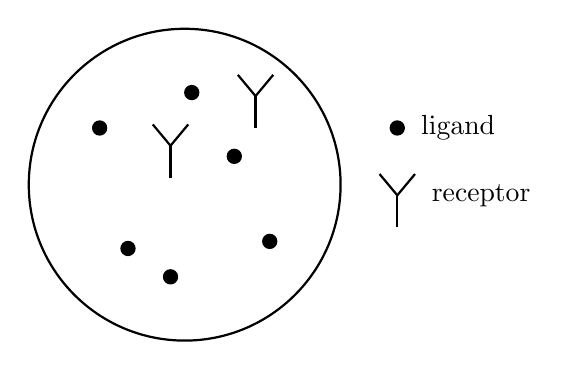
\begin{tikzpicture}[scale=0.9]

    % Volume
    \draw[thick] (0,0) circle (2.2);

    % Ligands
    \foreach \x/\y in {-1.2/0.8,-0.8/-0.9,0.1/1.3,0.7/0.4,1.2/-0.8,-0.2/-1.3} {
        \draw[fill=black] (\x,\y) circle (0.10);
    }

    % Receptor 1
    \draw[thick] (-0.2,0.1) -- (-0.2,0.55);
    \draw[thick] (-0.2,0.55) -- (-0.45,0.85);
    \draw[thick] (-0.2,0.55) -- (0.05,0.85);

    % Receptor 2
    \draw[thick] (1.0,0.8) -- (1.0,1.25);
    \draw[thick] (1.0,1.25) -- (0.75,1.55);
    \draw[thick] (1.0,1.25) -- (1.25,1.55);

    % Labels
    \draw[fill=black] (3.0,0.8) circle (0.10);
    \node[right] at (3.2,0.8) {ligand};

    \draw[thick] (3.0,-0.6) -- (3.0,-0.15);
    \draw[thick] (3.0,-0.15) -- (2.75,0.15);
    \draw[thick] (3.0,-0.15) -- (3.25,0.15);
    \node[right] at (3.35,-0.15) {receptor};

\end{tikzpicture}
\caption{A schematic volume containing ligands and receptors.}
\end{figure}

The continuous three-dimensional volume can be coarse-grained into a lattice of small volume elements.
For counting states, the same idea can be represented even more simply as a one-dimensional array of $\Omega$ boxes.

\begin{figure}[h!]
\centering
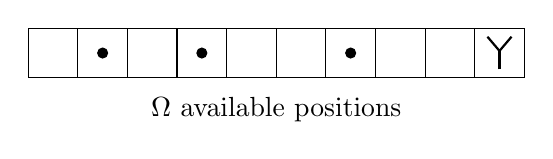
\begin{tikzpicture}[scale=0.9]

    \foreach \i in {0,...,9} {
        \draw (\i*0.7,0) rectangle ++(0.7,0.7);
    }

    % Ligands
    \draw[fill=black] (1.05,0.35) circle (0.07);
    \draw[fill=black] (2.45,0.35) circle (0.07);
    \draw[fill=black] (4.55,0.35) circle (0.07);

    % Receptor
    \draw[thick] (6.65,0.12) -- (6.65,0.38);
    \draw[thick] (6.65,0.38) -- (6.48,0.58);
    \draw[thick] (6.65,0.38) -- (6.82,0.58);

    \node at (3.5,-0.45) {$\Omega$ available positions};

\end{tikzpicture}
\caption{A simplified lattice representation of ligands and a receptor.}
\end{figure}


% ------------------------------------------------------------
\subsubsection*{i) Two boxes and one ligand}
% ------------------------------------------------------------

First consider the simplest possible system.
There is one ligand and one receptor, and the ligand can either remain unbound or occupy the receptor-binding state.

Choose the energy of the unbound state as the reference,
\[
    \epsilon_{\mathrm{unbound}}=0.
\]
The bound state has energy
\[
    \epsilon_{\mathrm{bound}}=\epsilon_b,
\]
with $\epsilon_b<0$ for energetically favorable binding.
The Boltzmann weights of the two states are therefore
\[
    w_{\mathrm{unbound}}=1,
\]
and
\[
    w_{\mathrm{bound}}=e^{-\beta\epsilon_b}.
\]
The partition function is
\[
    Z=1+e^{-\beta\epsilon_b}.
\]
The probability of being bound is therefore
\[
    p_b=\frac{e^{-\beta\epsilon_b}}{1+e^{-\beta\epsilon_b}}.
\]
Equivalently,
\[
    \frac{p_b}{1-p_b}=e^{-\beta\epsilon_b}.
\]


% ------------------------------------------------------------
\subsubsection*{ii) Many boxes and one ligand}
% ------------------------------------------------------------

Now suppose that an unbound ligand can occupy any of $\Omega$ equivalent solution positions.
There are therefore $\Omega$ distinct unbound microstates with energy zero, but only one bound state with energy $\epsilon_b$.

The total statistical weight of the unbound state is
\[
    W_{\mathrm{unbound}}=\Omega.
\]
The statistical weight of the bound state is
\[
    W_{\mathrm{bound}}=e^{-\beta\epsilon_b}.
\]
The partition function is
\[
    Z=\Omega+e^{-\beta\epsilon_b}.
\]
Therefore,
\[
    p_b=\frac{e^{-\beta\epsilon_b}}{\Omega+e^{-\beta\epsilon_b}}.
\]
This can be rewritten as
\[
    p_b=\frac{1}{1+\Omega e^{\beta\epsilon_b}}.
\]
Since
\[
    \Omega=e^{\ln\Omega},
\]
we can write
\[
    p_b=\frac{1}{1+\exp\left[\beta\left(\epsilon_b+k_BT\ln\Omega\right)\right]}.
\]
The quantity
\[
    \Delta F=\epsilon_b+k_BT\ln\Omega
\]
can be interpreted as the free-energy difference between the bound and unbound macrostates.

The energetic contribution $\epsilon_b<0$ favors binding.
The term $k_BT\ln\Omega>0$ represents the entropic cost of restricting a ligand that could otherwise occupy many different positions to a single bound state.
Binding therefore reflects a competition between energy and entropy.


% ------------------------------------------------------------
\subsubsection*{iii) Many boxes and many ligands}
% ------------------------------------------------------------

Now consider $L$ indistinguishable ligands and one receptor.
If the receptor is unbound, all $L$ ligands occupy solution positions.
The number of corresponding microstates is
\[
    W(L)=\binom{\Omega}{L}.
\]

If the receptor is bound, one ligand occupies the receptor and the remaining $L-1$ ligands occupy solution positions.
The number of corresponding solution microstates is therefore
\[
    W(L-1)=\binom{\Omega}{L-1}.
\]
The statistical weight of the unbound macrostate is
\[
    W_{\mathrm{unbound}}=W(L).
\]
The statistical weight of the bound macrostate is
\[
    W_{\mathrm{bound}}=W(L-1)e^{-\beta \epsilon_b}.
\]
Therefore,
\[
    p_b=\frac{W(L-1)e^{-\beta \epsilon_b}}{W(L)+W(L-1)e^{-\beta \epsilon_b}}.
\]
The ratio of multiplicities is
\[
    \frac{W(L-1)}{W(L)}=\frac{L}{\Omega-L+1}.
\]

For a dilute system in which $L \ll \Omega$,
\[
    \frac{W(L-1)}{W(L)} \approx \frac{L}{\Omega}.
\]
Hence
\[
    p_b \approx \frac{\frac{L}{\Omega}e^{-\beta \epsilon_b}}{1+\frac{L}{\Omega}e^{-\beta \epsilon_b}}.
\]

The ratio $L/\Omega$ plays the role of ligand concentration in the lattice model.
Thus increasing ligand concentration increases receptor occupancy.

This statistical-mechanical derivation produces the same general saturating form that appeared earlier in the mass-action treatment of ligand--receptor binding.


% ------------------------------------------------------------
\subsubsection*{Homework: active and inactive receptors}
% ------------------------------------------------------------

Extend the binding-by-counting argument to a receptor that can exist in both an active and an inactive state.
The receptor state introduces additional microstates and energetic contributions that must be included in the statistical weights.


% ============================================================

% Source: day4.tex:406; unit d4.4
\subsection{Two binding sites, interactions, and cooperativity}
\label{sec:two-receptors}


% ============================================================ 

The counting framework can also include interactions between receptors or between multiple binding sites on the same molecular complex.
Consider two binding sites and $L$ ligands.
Let $\epsilon_{\mathrm{sol}}$ denote the energy of an unbound ligand in solution, $\epsilon_b$ the binding energy of one ligand, and $\epsilon_{\mathrm{int}}$ an interaction energy that appears when both sites are occupied.
Table~\ref{tab:two-site-weights} enumerates the four possible occupancy states and gives their energies, multiplicities, and statistical weights.

\begin{table}[h!]
\centering
\renewcommand{\arraystretch}{1.5}
\begin{tabularx}{\textwidth}{
    |>{\centering\arraybackslash}p{2.5cm}
    |>{\raggedright\arraybackslash}X
    |>{\centering\arraybackslash}p{2.5cm}
    |>{\raggedright\arraybackslash}X|
}
\hline
\textbf{State} & \textbf{Energy} & \textbf{Multiplicity} & \textbf{Statistical weight}
\\
\hline
$Y \qquad Y$ &
$L\epsilon_{\mathrm{sol}}$ &
$W(L)$ &
$W(L)e^{-\beta L\epsilon_{\mathrm{sol}}}$
\\
\hline
$Y^{\circ} \qquad Y$ &
$(L-1)\epsilon_{\mathrm{sol}}+\epsilon_b$ &
$W(L-1)$ &
$W(L-1)e^{-\beta[(L-1)\epsilon_{\mathrm{sol}}+\epsilon_b]}$
\\
\hline
$Y \qquad Y^{\circ}$ &
$(L-1)\epsilon_{\mathrm{sol}}+\epsilon_b$ &
$W(L-1)$ &
$W(L-1)e^{-\beta[(L-1)\epsilon_{\mathrm{sol}}+\epsilon_b]}$
\\
\hline
$Y^{\circ} \qquad Y^{\circ}$ &
$(L-2)\epsilon_{\mathrm{sol}}+2\epsilon_b+\epsilon_{\mathrm{int}}$ &
$W(L-2)$ &
$W(L-2)e^{-\beta[(L-2)\epsilon_{\mathrm{sol}}+2\epsilon_b+\epsilon_{\mathrm{int}}]}$
\\
\hline
\end{tabularx}
\caption{States, energies, multiplicities, and statistical weights for two interacting binding sites.}
\label{tab:two-site-weights}
\end{table}

% If the two singly-bound states are grouped together into one macrostate, their total multiplicity is
% \[
%     2W(L-1).
% \]

As shown in Table~\ref{tab:two-site-weights}, there are two microscopically distinct singly bound states.
If these are grouped into one macrostate, their combined statistical weight is
\[
    2W(L-1)e^{-\beta[(L-1)\epsilon_{\mathrm{sol}}+\epsilon_b]}.
\]
The doubly bound state contains the additional interaction energy $\epsilon_{\mathrm{int}}$.
If $\epsilon_{\mathrm{int}}<0$, simultaneous occupancy is energetically favored, producing positive cooperativity.
If $\epsilon_{\mathrm{int}}>0$, simultaneous occupancy is energetically penalized, producing negative cooperativity.

% ============================================================

% Source: day4.tex:467; unit d4.5
\subsection{Case study: reading a Bicoid concentration gradient}
\label{sec:bicoid}


% ============================================================

Bicoid is a transcription factor that forms a concentration gradient along the anterior--posterior axis of the early \textit{Drosophila} embryo \cite{driever1988gradient}.
Bicoid regulates target genes such as \textit{hunchback}, and the local Bicoid concentration helps determine where these genes are expressed \cite{driever1989bicoid,driever1989determination}.
This provides a biological example in which a spatial concentration profile is translated through concentration-dependent regulatory binding into a spatial pattern of gene expression.


% ============================================================

% EDITORIAL ADDITION: navigation or conceptual bridge
% This example connects a spatial profile to a local binding response.
% The original notes discuss that readout but do not derive a dynamical model for generating the Bicoid gradient.
% Source: day4.tex:476; unit d4.6


\subsection{Allostery: the second secret of life}
\label{sec:allostery}


% ============================================================

The word \emph{allostery} comes from the Greek \emph{allos}, meaning ``other'', and \emph{stereos}, meaning ``solid'' or ``structure''.
In an allosteric protein, a regulatory molecule binds at a site that is physically distinct from the protein's active or functional site.
Binding at the regulatory site changes the energetic or conformational state of the protein and thereby alters activity at the other site \cite{monod1963allosteric}.
The central idea is therefore coupling between spatially distinct sites on the same molecular system.

Allosteric regulation of this kind is widespread in biology.
Metabolic pathways provide many examples in which metabolites regulate enzymes upstream or downstream in the pathway \cite{monod1963allosteric}.
Glycolysis, which converts glucose into pyruvate, contains several such regulatory steps.

Allostery provides a molecular mechanism through which a protein can sense one chemical signal and alter its response to another.

% ------------------------------------------------------------
\subsubsection{Statistical mechanics of allosteric enzymes}
% ------------------------------------------------------------

A useful framework for describing allosteric enzymes is the Monod-Wyman-Changeux (MWC) model \cite{monod1965nature}.
In this picture, an enzyme can fluctuate between different conformational states, commonly an active state and an inactive state.
These states can have different substrate-binding affinities and different catalytic activities.
The relative probabilities of the states, together with ligand binding, determine the overall activity of the enzyme.

The same states-and-weights idea used for ligand binding can therefore be extended to allostery.
Instead of considering only bound and unbound states, we enumerate combinations of conformational state and ligand occupancy, assign each state an appropriate statistical weight, and normalize over all possible states.

Einav, Mazutis, and Phillips developed this states-and-weights treatment into a statistical-mechanical framework for allosteric enzymes \cite{einav2016statistical}.
Their formulation first recasts Michaelis--Menten kinetics in terms of enzyme states and statistical weights and then extends the framework to MWC enzymes, allosteric regulators, competitive inhibitors, and enzymes with multiple substrate-binding sites.